\begin{figure}[!htbp]
\centering
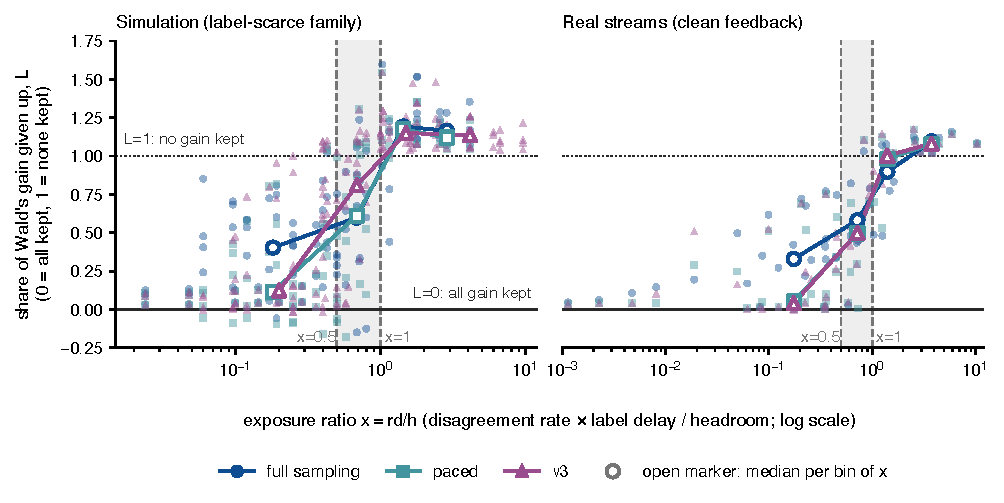
\includegraphics[width=\linewidth]{figures/fig_regime_map.pdf}
\caption{For the paced variants, median $L$, the share of the unconstrained rule's improvement given up, is small when $x=rd/h<0.5$ and close to 1 when $x\ge1$. Each point is one evaluated unit (regime or stream, shield arm, headroom $h$) where Wald with cutoff gains at least 10\% of the cost of never switching. Here $x$ is disagreement rate times label delay divided by headroom; $L=0$ means the whole gain is kept and $L=1$ that none is. Values $L<0$ mean the shield is cheaper than Wald, while $L>1$ means it costs more than never switching. Left: label-scarce simulation family; right: ten real streams with clean feedback. Open markers show bin medians for $[0,.5)$, $[.5,1)$, $[1,2)$ and $[2,\infty)$; lines join those medians and are not a fitted law. The shaded band marks $.5\le x<1$. Source: \texttt{exposure\_ratio\_test.json}.}
\label{fig:regime_map}
\end{figure}
